\section{Лекція 12: Помилки та виключення}
 
 \subsection{Вступ в обробку виключень} 
\begin{frame}
% \frametitle{Логічні висновки}
Виключення бувають:
\begin{itemize}
  \item в процесі виконання програми (можна оброблювати);
  \item в процесі компіляції програми (треба правильно писати програму).
\end{itemize}

\texttt{try:}

\texttt{~~~~operations\_1}

\texttt{except error\_1:}

\texttt{~~~~operations\_2}

\texttt{except error\_2:}

\texttt{~~~~operations\_3}

При <<відловлюванні>> виключень враховується ієрархія класів виключень.
\end{frame}

\begin{frame}
\begin{figure}
\begin{center}
 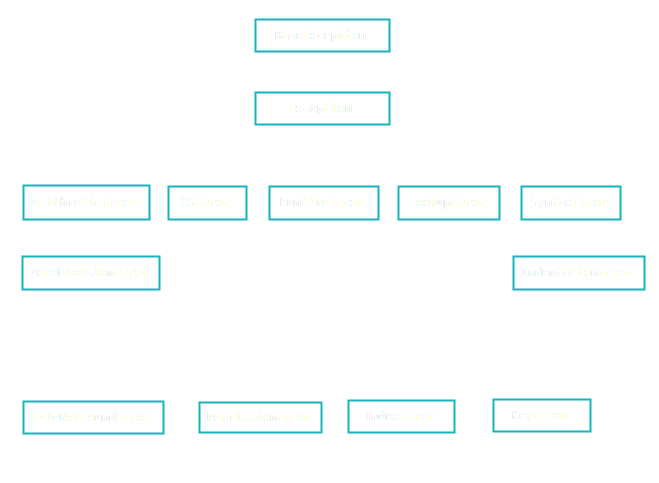
\includegraphics[width=0.75\textwidth]{pictures/exception.png}
\caption{Виключення}
\label{exception} 
\end{center}
\end{figure}

\end{frame}

\begin{frame}
% \frametitle{Логічні висновки}
\texttt{try:}

\texttt{~~~~operations\_1}

\texttt{except error\_1 as val:}

\texttt{~~~~operations\_2}

\texttt{else:}

\texttt{~~~~operations\_3}

\texttt{finally:}

\texttt{~~~~operations\_4}

\texttt{val} - посилання на екземпляр класу виключення. Блок коду після оператору \texttt{else} виконується при штатному завершенні блоку після оператора \texttt{try}. Блок коду після оператору \texttt{finally} виконується завжди (до оператора \texttt{return}).
\end{frame}
